\section{Results}

%\song{Update all papers including all papers in 2022} \nima{done}

We present our analyses and findings in this section to address the research questions we devised in Section~\ref{sec:intro}. 

\subsection{RQ1. What is the trend of studies using ML/DL models for vulnerability detection?}

To comprehend the trend of publications, we examined the publication dates along with the venues in which they were presented.

\subsubsection{RQ1.1. What are the trends of studies in software vulnerability detection over time?}
%In this paper, we analyzed studies published between 2011 and 2022 to characterize the trend of studies for software vulnerability detection. 
Figure~\ref{fig:pub_trends} %\jie{this figure is far away from here, a little hard to find it.} \nima{done} \song{please fix the same issue globally, should always keep the table/fig close to their first reference} \nima{I will fix this issue at the end when I finished adding contents, because if I add or remove contents, the order may be changed again.} 
demonstrates the publication trend of vulnerability detection studies published in eleven years, i.e., between 2011 and 2022. It is observable that the number of publications has increased gradually over the years. There is only one publication from 2011 to 2016, and the number of publications increased to 18 in 2021. However, there is a decrease in the number of publications in 2022 compared to the previous year. We have also examined the cumulative number of publications shown in Figure \ref{fig:pub_trends}. It is noticeable that the curve fitting the distribution shows a significant increase in slope between 2018 and 2022 %, indicating that there is a substantial increase in the number of relevant studies using DL for vulnerability detection in the future. 
suggesting that the use of ML/DL techniques for software vulnerability detection has become a prevalent trend since 2017, and a broad range of studies have utilized ML/DL models to address challenges in this field.


\begin{figure}[t!]
\centering
\begin{subfigure}{.5\textwidth}
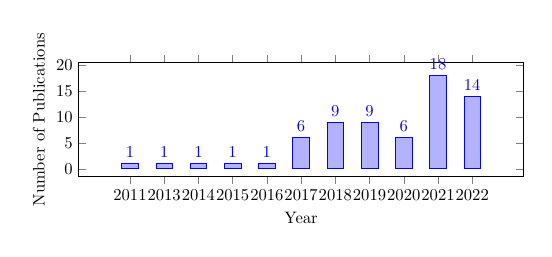
\begin{tikzpicture}[scale=0.6]
\begin{axis}  
[  
    ybar,  
    enlargelimits=0.15,  
    width=11cm,
    height=4cm,
    ylabel={Number of Publications}, 
    xlabel={Year},  
    symbolic x coords={2011, 2013, 2014,2015,2016, 2017, 2018, 2019, 2020, 2021, 2022}, 
    xtick=data,  
     nodes near coords,
    nodes near coords align={vertical},  
    ]  
\addplot coordinates {
(2022, 14)
(2021, 18)
(2020, 6)
(2019,9)
(2018,    9)
(2017,   6)
(2016,   1)
(2015,    1)
(2014,   1)
(2013,   1)
(2011,1)
};  
\end{axis}  
\end{tikzpicture}
\label{fig:pub_trends1}
\end{subfigure}%
\begin{subfigure}{.5\textwidth}
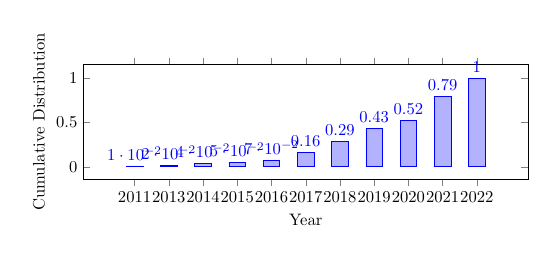
\begin{tikzpicture}[scale=0.6]
\begin{axis}  
[  
    ybar,  
    enlargelimits=0.15,  
    width=11cm,
     height=4cm,
    ylabel={Cumulative Distribution}, 
    xlabel={Year},  
    symbolic x coords={2011, 2013, 2014, 2015,2016, 2017, 2018, 2019, 2020, 2021, 2022}, 
    xtick=data,  
     nodes near coords,
    nodes near coords align={vertical},  
    ]  
\addplot coordinates {
(2011,0.01)
(2013,0.02)
(2014,0.04)
(2015,0.05)
(2016,0.07)
(2017,0.16)
(2018,0.29)
(2019,0.43)
(2020,0.52)
(2021,0.79)
(2022,1)
};  
\end{axis}  
\end{tikzpicture}
\label{fig:pub_trends2}
\end{subfigure}%
\newline
\caption{Publication trend of vulnerability detection studies.}
\label{fig:pub_trends}
\end{figure}
% \song{value of 2021 should not be 1} \nima{working on this}}

\begin{table}[t!]
\caption{Conference publication venues for manual search.}
\renewcommand{\arraystretch}{0.3}
\resizebox{\columnwidth}{!}{%
\begin{tabular}{ccl}
\toprule
No & Acronym & Full name                                                               \\
\midrule
1  & ICSE    & International Conference on Software Engineering                        \\
2  & ECSE/FSE & ACM SIGSOFT Symposium on the Foundation of Software Engineering \\
3 & ASE     & IEEE/ACM International Conference on Automated Software Engineering     \\
4 & USENIX  & USENIX                 \\
5  & OOPSLA   & Object-oriented Programming, Systems, Languages, and Applications      \\
6 & ISSTA & ACM SIGSOFT International Symposium on Software Testing and Analysis \\
7  & MSR     & IEEE Working Conference on Mining Software Repositories                 \\
8 & SANER & IEEE International Conference on Software Analysis, Evolution and Reengineering \\
9  & ISSRE   & IEEE International Symposium on Software Reliability Engineering        \\
10 & ICSME   & IEEE International Conference on Software Maintenance and Evolution     \\
11  & IJCAI   & International Joint Conferences on Artificial Intelligence Organization \\
12  & CCS     & ACM SIGSAC Conference on Computer and Communications Security           \\
13  & ICLR    & International Conference on Learning Representations                    \\
14  & NIPS    & International Conference on Neural Information Processing Systems       \\
15 & MASCOT   & Modelling, Analysis, and Simulation of Computer and Telecommunication Systems                            \\
16 & QRS     & IEEE International Conference on Software Security and Reliability      \\
17 & KDDM    & Pacific-Asia Conference on Knowledge Discovery and Data Mining          \\
18 & NDSS    & Network and Distributed Systems Security Symposium               \\
19 & ARES    & ACM International Conference on Availability, Reliability and Security  \\
20 & INFOCOM & IEEE International Workshop on Security and Privacy in Big Data         \\
21 & ICTAI   & IEEE International Conference on Tools with Artificial Intelligence     \\
22 & ICDM    & IEEE International Conference on Data Mining                            \\
23 & GLOBCOM & IEEE Global Communications Conference                                   \\
24 & TrustCom & IEEE International Conference on Trust, Security and Privacy in Computing and Communications \\
25 & DSAA & IEEE International Conference on Data Science and Advanced Analytic \\
\bottomrule
\end{tabular}}
\label{tbl:confLegend}
\end{table}
\begin{table}[h]
\caption{Journal publication venues for manual search.}
%\renewcommand{\arraystretch}{0.3}
{%
\begin{tabular}{ccl}
\toprule
No & Journal Acronym & Full Name                                               \\
\midrule
1  & TSE             & IEEE Transaction on Software Engineering                \\
2  & TOSEM           & ACM Transaction on Software Engineering and Methodology     \\
3  & IST             & Information and Software Technology                     \\
4  & ESM             & Empirical Software Engineering                          \\
5  & JSS             & Journal of System and Software                         \\
6  & TDSC            & IEEE Transaction on Dependable and Secure Computing     \\
7  & CSJ             & Computer and Security Journal                           \\
8  & TIFS            & IEEE Transactions on Information Forensics and Security \\
9  & ISJ             & Information Sciences Journal                            \\
10 & TFS             & IEEE Transaction on Fuzzy Systems                       \\
11 & TKDE            & IEEE Transaction on Knowledge and Data Engineering \\
12 & KBS             & Knowledge-Based Systems \\
\bottomrule
\end{tabular}}
\label{tbl:jourLegend}
\end{table}

% \song{Table 2 and 3 are not mentioned in part of your paper, please do read want you write!!!!} \nima{done}




\subsubsection{RQ1.2: What is the distribution of the publication venues?}
In this study, overall, we analyzed and reviewed 67 papers from various publication venues including 43 conference and symposium papers along with 24 journal papers. We have included the conference and journal acronyms and their complete names for reference in Table \ref{tbl:confLegend} and Table \ref{tbl:jourLegend}. Table \ref{tbl:venueDist}
% \song{too far, move it here; do not skip table ids, there are table 2 and 3 in between} \nima{done} 
shows the distribution of primary studies for each publication venue. 64.1\% of publications are published in conferences and symposiums while 35.8\% of papers have been published as journal papers. It is observable that MSR, IJCAI, and ECSE/FSE are the most popular venues that have the highest number of primary studies, each of which contains 4 papers. %It is worth mentioning that IJCAI which is not a SE venue has more vulnerability detection papers than top SE venues including ICSE, ASE, and ECSE/FSE. 
Meanwhile, among the journals, TDSC and TSE include the highest number of studies, i.e., 6 and 4 studies respectively.

\mybox{Answer to RQ1}{red!40}{gray!10}{
(1) The results indicate that the application of ML/DL techniques for software vulnerability detection has had a remarkable rising trend in the past few years.\\
(2) A large proportion of papers are published in recent two years, i.e., 2021 and 2022.\\
% (3) The number of conference papers that addressed the problem of software vulnerability detection is larger than the number of corresponding journal papers. \jie{In my opinion, this comparison might not fair since you search 25 conferences, and only 12 journals. for example you include the ASE conference, yet not include the ASE journal. I think it might be better to remove this point in the summary.}\\
(3) MSR, IJCAI, and ECSE/FSE are the most popular conference venues. On the other hand, TDSC and TSE are the most popular journal venues.\\
}


\begin{table}[h]
\caption{Distribution of publications based on conference and journal venues.}
\setlength\tabcolsep{2.0pt}
\begin{tabular}{lcclcc}
\toprule
Conference Venue & \# Studies & References & Journal Venue         & \# Studies & References \\
\midrule
MSR   & 4          &  \cite{chen2020machine, hoang2019deepjit, hin2022linevd, fu2022linevul}    & TDSC & 6  &   \cite{liu2020cd, zou2019mu, lin2019software, li2021sysevr, li2021vuldeelocator, zou2022mvulpreter}         \\
IJCAI            & 4          &    \cite{3172102, zhuang2020smart, duan2019vulsniper, liu2021smart}        & TSE & 4            &     \cite{dam2018automatic, dam2017automatic, chen2021neural, scandariato2014predicting}       \\
ECSE/FSE         & 4          &   \cite{zhou2017automated, li2021vulnerability, ni2022best, nguyen2022mando}      & CSJ & 2 &      \cite{jeon2021autovas, yan2021han}      \\
CCS              & 3          &       \cite{yamaguchi2013chucky, lin2017poster, perl2015vccfinder, cheng2019static}      & IST   & 2   &   \cite{shippey2019automatically, tian2020bvdetector}         \\
 ISSRE            & 3          &     \cite{zheng2021vulspg, wu2021peculiar, zeng2021gcn2defect}           & TIFS    & 2 &    \cite{wang2020combining, huang2021hunting}        \\
ICLR             & 2          &    \cite{dinella2020hoppity, le2018maximal}        & TOSEM & 2 &   \cite{cheng2021deepwukong, 3429444}         \\
ICSE             & 2          &   \cite{cao2022mvd, wang2016automatically}          & ESM  & 1 &    \cite{riom2021revisiting}        \\
OOPSLA           & 2          &    \cite{pradel2018deepbugs, 3360588}        & ISJ  & 1  & \cite{ghaffarian2021neural}   \\
NIPS             & 2          &         \cite{3327890, zhou2019devign}   & JSS  & 1  &  \cite{pascarella2019fine}          \\
  ASE         & 2          &      \cite{le2021deepcva, zhang2022reentrancy}      & TFS & 1  &  \cite{liu2019deepbalance} \\
QRS              & 1          &        \cite{li2017software}    & TKDE   & 1   &   \cite{liu2021combining}         \\
KDDM             & 1          &      \cite{nguyen2020deep}      & KBS  &  1 &   \cite{zhuang2022just}   \\
NDSS             & 1          &       \cite{li2018vuldeepecker}     &  \textbf{SUM}   & \textbf{24}  &       \\
ARES             & 1          &       \cite{kronjee2018discovering}     &     &   &      \\
INFOCOM          & 1          &     \cite{ziems2021security}       &       &   &       \\
MASCOT               & 1          &    \cite{filus2020random}          &   &  &       \\
ICTAI            & 1          &      \cite{phan2017convolutional}      &    &   &            \\
ICSME            & 1          &      \cite{sabetta2018practical}      &      &       &            \\
ICDM             & 1          &       \cite{8594942}     &    &            &    \\
GLOBCOM          & 1          &      \cite{Vuldiggerpaper}      &          &       &            \\
USENIX           & 1          &     \cite{yamaguchi2011vulnerability}    &  &           &             \\
DSAA             & 1          &     \cite{nguyen2022mando}    &  &           &             \\
ISSTA            & 1          &     \cite{cheng2022path}    &  &           &             \\
SANER            & 1          &     \cite{ding2022velvet}    &  &           &             \\
TrustCom         & 1          &     \cite{yang2022source}    &  &           &             \\
\textbf{SUM} & \textbf{43} & & & &  \\
\bottomrule
\end{tabular}
\label{tbl:venueDist}
\end{table}

% \begin{figure}[H]
%     \centering
%      {\includegraphics{Figures/distribution_conf.png}}
%      \caption{Number of publications per year}
%     \label{pub_per_year}
% \end{figure}

% \begin{figure}[H]
% \centering
% \begin{subfigure}{.5\textwidth}
%   \centering
%   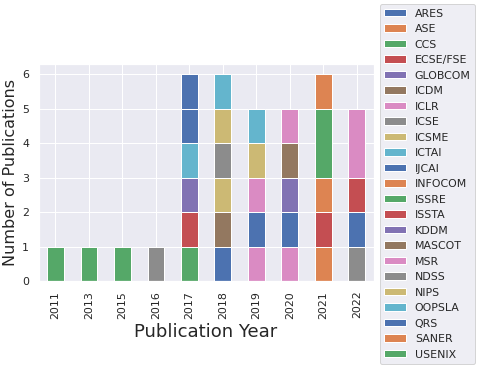
\includegraphics[width=0.9\linewidth]{Figures/RQ1/distribution_conf.png}
%   \caption{Number of studies published in various conferences.}
%   \label{fig:venue1}
% \end{subfigure}%
% \begin{subfigure}{.5\textwidth}
%   \centering
%   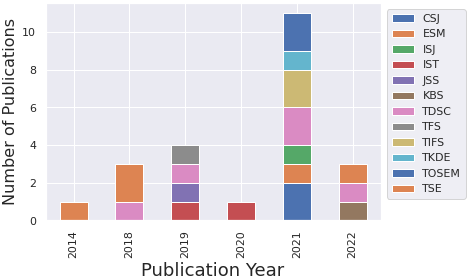
\includegraphics[width=1.2\linewidth]{Figures/RQ1/distribution_jour.png}
%   \caption{Number of studies published in various journals.}
%   \label{fig:venue2}
% \end{subfigure}%
% \newline
% \caption{Distribution of different publication venues.}
% \label{fig:pub_venues}
% \end{figure}

       %  xticklabels={ {ARES}, {ASE}, {CCS}, {ECSE/FSE}, {GLOBCOM}, {ICDM}, {ICLR},
       % {ICSE}, {ICSME}, {ICTAI}, {IJCAI}, {INFOCOM}, {ISSRE}, {ISSTA},
       % {KDDM}, {MASCOT}, {MSR}, {NDSS}, {NIPS}, {OOPSLA}, {QRS}, {SANER},
       % {USENIX}},
% \definecolor{ForestGreen}{RGB}{34,139,34}
% \pgfplotstableread{
% PublicationYear	2011 	2013 	2015 	2016 	2017 	2018 	2019 	2020 	2021 	2022
% ASE 	0 	0 	0 	0 	0 	0 	0 	0 	1 	0
% CCS 	0 	1 	1 	0 	1 	0 	0 	0 	0 	0
% ECSE/FSE 	0 	0 	0 	0 	1 	0 	0 	0 	1 	0
% ICDM 	0 	0 	0 	0 	0 	1 	0 	0 	0 	0
% ICLR 	0 	0 	0 	0 	0 	0 	1 	1 	0 	0
% ICSE 	0 	0 	0 	1 	0 	0 	0 	0 	0 	1
% IJCAI 	0 	0 	0 	0 	1 	0 	1 	1 	0 	1
% INFOCOM 	0 	0 	0 	0 	0 	0 	0 	0 	1 	0
% ISSTA 	0 	0 	0 	0 	0 	0 	0 	0 	0 	1
% NDSS 	0 	0 	0 	0 	0 	1 	0 	0 	0 	0
% NIPS 	0 	0 	0 	0 	0 	1 	1 	0 	0 	0
% OOPSLA 	0 	0 	0 	0 	0 	1 	1 	0 	0 	0
% USENIX 	1 	0 	0 	0 	0 	0 	0 	0 	0 	0
% }\testdata
% \begin{figure}[t!]
% \centering
% \renewcommand{\arraystretch}{1}
% \resizebox{0.6\columnwidth}{!}{%
%     \begin{tikzpicture}[scale=0.6]
%     \begin{axis}[
%         ybar stacked,
%     	bar width=15pt,
%         ymin=0,
%         ymax=5,
%         xtick=data,
%         legend style={at={(1.01,0.6)},anchor=west},
%         reverse legend=true,
%         %yticklabels from table={\testdata}{Label},
%         xticklabels={ {ASE}, {CCS}, {ECSE/FSE}, {ICDM}, {ICLR}, {ICSE}, {IJCAI},
%        {INFOCOM}, {ISSTA}, {NDSS}, {NIPS}, {OOPSLA},{USENIX}},
%         xticklabel style={rotate=25,anchor=east},
%     ]
%     \addplot + [ nodes near coords, fill=green!80]      table    [y=2011, meta=Label, x expr=\coordindex] {\testdata};
%     \addplot + [nodes near coords, fill=blue!60]         table    [y=2013, meta=Label, x expr=\coordindex] {\testdata};
%     \addplot + [nodes near coords, fill=red!60]         table    [y=2015, meta=Label, x expr=\coordindex] {\testdata};
%     \addplot + [nodes near coords, fill=ForestGreen!60] table    [y=2016, meta=Label, x expr=\coordindex] {\testdata};
%     \addplot + [nodes near coords, fill=yellow!60]      table    [y=2017, meta=Label, x expr=\coordindex] {\testdata};
%     \addplot + [nodes near coords, fill={rgb:red,1;green,2;blue,5}] table [y=2018, meta=Label, x expr=\coordindex] {\testdata};
%     \addplot + [nodes near coords, fill={rgb:blue,1;yellow,2;pink,5}] table    [y=2019, meta=Label, x expr=\coordindex] {\testdata};
%     \addplot + [nodes near coords, fill={rgb:yellow,1;red,2;pink,5}] table    [y=2020, meta=Label, x expr=\coordindex] {\testdata};
%     \addplot + [nodes near coords, fill={rgb:pink,1;yellow,2;orange,5}] table    [y=2021, meta=Label, x expr=\coordindex] {\testdata};
%     \addplot + [nodes near coords, fill={rgb:orange,1;blue,2;pink,5}] table    [y=2022, meta=Label, x expr=\coordindex] {\testdata};
% \legend{2011,
% 2013,
% 2015,
% 2016,
% 2017,
% 2018,
% 2019,
% 2020,
% 2021,
% 2022
% }
% \end{axis}
% \end{tikzpicture}}
% \caption{The distribution of software vulnerabilities in the studied ML libraries.}
% \label{typeDist}
% \end{figure}

\definecolor{airforceblue}{rgb}{0.36, 0.54, 0.66}
\definecolor{aliceblue}{rgb}{0.94, 0.97, 1.0}
\definecolor{alizarin}{rgb}{0.82, 0.1, 0.26}
\definecolor{almond}{rgb}{0.94, 0.87, 0.8}
\definecolor{amaranth}{rgb}{0.9, 0.17, 0.31}
\definecolor{amber}{rgb}{1.0, 0.75, 0.0}
\definecolor{amber(sae/ece)}{rgb}{1.0, 0.49, 0.0}
\definecolor{americanrose}{rgb}{1.0, 0.01, 0.24}
\definecolor{amethyst}{rgb}{0.6, 0.4, 0.8}
\definecolor{anti-flashwhite}{rgb}{0.95, 0.95, 0.96}
\definecolor{antiquebrass}{rgb}{0.8, 0.58, 0.46}
\definecolor{antiquefuchsia}{rgb}{0.57, 0.36, 0.51}



% \pgfplotstableread{
% ASE	ICLR	USENIX	ISSRE	SANER	IJCAI	ICSME	ISSTA	ICDM	ICTAI	ARES	MSR	OOPSLA	CCS	NIPS	ICSE	ECSE/FSE
% 2020 0	1	0	0	0	1	0	0	0	0	0	1	0	0	0	0	0
% 2013 0	0	0	0	0	0	0	0	0	0	0	0	0	1	0	0	0
% 2022 1	0	0	0	0	1	0	1	0	0	0	2	0	0	0	1	2
% 2011 0	0	1	0	0	0	0	0	0	0	0	0	0	0	0	0	0
% 2018 0	0	0	0	0	0	1	0	1	0	1	0	1	0	1	0	0
% 2015 0	0	0	0	0	0	0	0	0	0	0	0	0	1	0	0	0
% 2021 1	0	0	2	1	0	0	0	0	0	0	0	0	0	0	0	1
% 2019 0	1	0	0	0	1	0	0	0	0	0	1	1	0	1	0	0
% 2017 0	0	0	0	0	1	0	0	0	1	0	0	0	1	0	0	1
% 2016 0	0	0	0	0	0	0	0	0	0	0	0	0	0	0	1	0
% }\testdata
% \begin{figure}[H]
% \centering
% \begin{subfigure}{.5\textwidth}
% \centering
% \begin{tikzpicture}[scale=0.6]
% \begin{axis}[
%         ybar stacked,
%     	bar width=15pt,
%         ymin=0,
%         ymax=5,
%         xtick=data,
%         legend style={at={(1.01,0.54)},anchor=west},
%         reverse legend=true,
%         %yticklabels from table={\testdata}{Label},
%         xticklabels={ {2011}, {2013}, {2015}, {2016}, {2017}, {2018}, {2019},
%        {2020}, {2021}, {2022}},
%         xticklabel style={rotate=25,anchor=east},
%     ]
%     \addplot + [ nodes near coords, fill=green!80]      table    [y=ASE, meta=Label, x expr=\coordindex] {\testdata};
%     \addplot + [nodes near coords, fill=blue!60]         table    [y=CCS, meta=Label, x expr=\coordindex] {\testdata};
%     \addplot + [nodes near coords, fill=red!60]         table    [y=ECSE/FSE, meta=Label, x expr=\coordindex] {\testdata};
%     \addplot + [nodes near coords, fill=ForestGreen!60] table    [y=ICDM, meta=Label, x expr=\coordindex] {\testdata};
%     \addplot + [nodes near coords, fill=yellow!60]      table    [y=ICLR, meta=Label, x expr=\coordindex] {\testdata};
%     \addplot + [nodes near coords, fill={antiquefuchsia}] table [y=ICSE, meta=Label, x expr=\coordindex] {\testdata};
%     \addplot + [nodes near coords, fill={airforceblue}] table    [y=IJCAI, meta=Label, x expr=\coordindex] {\testdata};
%     \addplot + [nodes near coords, fill={aliceblue}] table    [y=INFOCOM, meta=Label, x expr=\coordindex] {\testdata};
%     \addplot + [nodes near coords, fill={alizarin}] table    [y=ISSTA, meta=Label, x expr=\coordindex] {\testdata};
%     \addplot + [nodes near coords, fill={almond}] table    [y=NIPS, meta=Label, x expr=\coordindex] {\testdata};
%     \addplot + [nodes near coords, fill={amaranth}] table    [y=OOPSLA, meta=Label, x expr=\coordindex] {\testdata};
%     \addplot + [nodes near coords, fill={amber}] table    [y=USENIX, meta=Label, x expr=\coordindex] {\testdata};
% \legend{ASE,
% CCS,
% ECSE/FSE,
% ICDM,
% ICLR,
% ICSE,
% IJCAI,
% INFOCOM,
% ISSTA,
% NIPS,
% OOPSLA,
% USENIX
% }
% \end{axis}
% \end{tikzpicture}
% \caption{Number of studies published in various conferences.}
% \label{fig:venue1}
% \end{subfigure}%
% \pgfplotstableread{
% PublicationYear TFS	TKDE TOSEM TSE
% 2014 	0 	0 	0 	1
% 2018 	0 	0 	0 	2
% 2019 	1 	0 	0 	0
% 2021 	0 	1 	2 	0
% 2022 	0 	0 	0 	1
% }\testdata
% \begin{subfigure}{.5\textwidth}
% \centering
% \begin{tikzpicture}[scale=0.6]
% \begin{axis}[
%         ybar stacked,
%     	bar width=15pt,
%         ymin=0,
%         ymax=5,
%         xtick=data,
%         legend style={at={(1.01,0.54)},anchor=west},
%         reverse legend=true,
%         %yticklabels from table={\testdata}{Label},
%         xticklabels={ {2014}, {2018}, {2019}, {2021}, {2022}},
%         xticklabel style={rotate=25,anchor=east},
%     ]
%     \addplot + [ nodes near coords, fill=green!80]      table    [y=TFS, meta=Label, x expr=\coordindex] {\testdata};
%     \addplot + [nodes near coords, fill=blue!60]         table    [y=TKDE, meta=Label, x expr=\coordindex] {\testdata};
%     \addplot + [nodes near coords, fill=red!60]         table    [y=TOSEM, meta=Label, x expr=\coordindex] {\testdata};
%     \addplot + [nodes near coords, fill=ForestGreen!60] table    [y=TSE, meta=Label, x expr=\coordindex] {\testdata};
% \legend{TFS,
% TKDE,
% TOSEM,
% TSE
% }
% \end{axis}
% \end{tikzpicture}
% \caption{Number of studies published in various journals.}
% \label{fig:venue2}
% \end{subfigure}%
% \newline
% \caption{Distribution of different publication venues.}
% \label{fig:pub_venues}
% \end{figure}





